
\documentclass{article}

\title{Good names form Galois connections}
\subtitle{A quest for defining what it means to name things well.}
\date{2024-04-01}
\modified{2024-04-01}
\keyword{glasperlenspiel}

\begin{document}

\section*

\epigraph{
    You can know the name of that bird in all the languages of the world, but when you're finished, you'll know absolutely nothing whatever about the bird.
    You'll only know about humans in different places, and what they call the bird.
    So let's look at the bird and see what it's doing---that's what counts. 
}{Richard Feynman, ``What Do You Care What Other People Think?''}

I recently read a chapter on naming things in ``\href{https://www.goodreads.com/book/show/57196550-the-programmer-s-brain}{The Programmer's Brain}'' by Felienne Hermans.
There is a lot of research on the topic of names in programming.
Researchers found that good names improve code comprehension and that \href{https://oro.open.ac.uk/17007/1/butler09wcreshort_latest.pdf}{poor names correlate with buggy code}
and proposed a few heuristics for choosing good names\sidenote{mn-naming-heuristics}{
  See, for example, ``\href{https://arxiv.org/pdf/2103.07487.pdf}{How Developers Choose Names}'' by Dror G. Feitelson et al.,
  and ``\href{https://ieeexplore.ieee.org/abstract/document/5090039}{To camelcase or to under_score}'' by Dave Binkey et al.
}.

The book provides a few recommendations on how to create good names\sidenote{mn-naming-books}{
  There are many books with naming heuristics ranging from classics such as ``\href{https://www.goodreads.com/book/show/4845.Code_Complete}{Code Complete}'' by Steve McConnell and ``\href{https://www.goodreads.com/book/show/3735293-clean-code}{Clean Code}'' by Robert C. Martin
  to more recent ``\href{https://www.goodreads.com/book/show/123009242-naming-things}{Naming things.}'' by Tom Benner.
}, but it left me unsatisfied.
I felt that I already knew \em{how} to choose good names, but I wanted to have a good mathematical model for what good names \em{are}.
This article is the result of my exploration.

\section{objects-concepts-expressions}{Objects, concepts, and expressions}

\epigraph{
  I will defend the thesis that thought has a kind of priority over words and that the concept has a kind of priority over its expression.
}{Johan Granström, ``Tretise on Intuitionistic Type Theory'', p. 2}

In the beginning was the Word.
No, scratch that.
There is overwhelming evidence that the world existed for billions of years before our ancestors uttered their first words.
In the beginning was the Thing.

But then came the Word, right? Nah.
Living creatures created mental models of their environments long before the first language appeared.
Even soulless and speechless neural networks seem to recognize concepts (such as \href{https://github.com/rcgc/chihuahua-muffin}{``Chihuahua'' or ``muffin''}) in raw sensory input.
The Concept came after the Thing.

Unfortunately, concepts are internal to the mind holding them.
Until we figure out how to make \href{https://en.wikipedia.org/wiki/Telepathy}{telepathy} work, we must use some encoding to communicate concepts between minds.
That's where the Word comes into the picture.
Words are arbitrary symbols representing concepts.

I'll borrow terminology from \href{https://link.springer.com/book/10.1007/978-94-007-1736-7}{Tretise on Intuitionistic Type Theory} and use
\em{object} to refer to things existing in the world (we won't need them much, though),
\em{concept} to refer to mental representations of these objects,
and \em{expression} to refer to words or sentences used to communicate concepts.

\begin{figure}[grayscale-diagram]
  \marginnote{mn-object-concept-expression}{
    The relationship between an object (fluffy the cat), a concept (the idea of a cat in mind), and its expression (the word ``cat'').
  }
  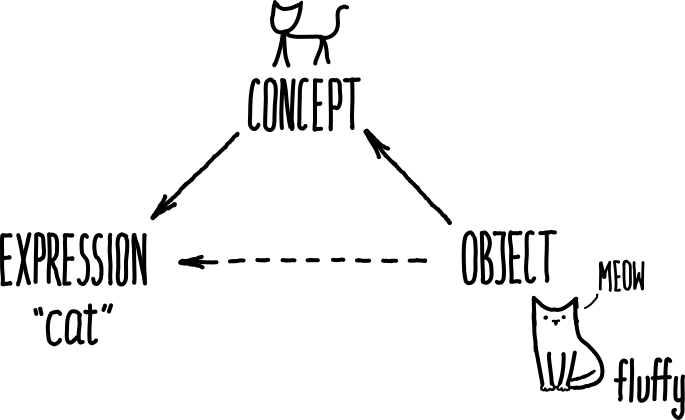
\includegraphics{/images/26-object-concept-expression.svg}
\end{figure}

\section{maps-of-meaning}{Maps of meaning}

The distinction between objects, concepts, and expressions is almost as old as Western philosophy.
Unfortunately, it misses one crucial point: concepts and their expressions don't map one-to-one.
Most concepts have multiple expressions; most words map to several concepts (any dictionary is living proof).
For example, consuming food can be labeled as ``eating'' or ``dining''.
And the word ``go'' can refer to walking or a board game.
More precisely, expressions and concepts form a \href{https://en.wikipedia.org/wiki/Binary_relation}{binary relation}.

\begin{figure}[grayscale-diagram,medium-size]
  \marginnote{mn-concepts-words}{
    The relationship between concepts and words is many-to-many: different words can express the same concept, and unrelated concepts can map to the same word.
  }
  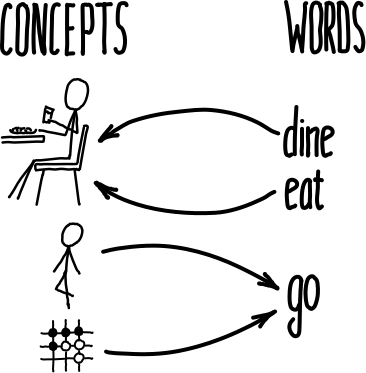
\includegraphics{/images/26-concepts-words.svg}
\end{figure}

We must add another ingredient to the picture to tackle the problem of names: the \em{context}.
Context refers to all the other things that influence the interpretation of an expression: surrounding words in the sentence, the task the reader is trying to accomplish, and the reader's culture and background.
The amount of information in the context is vast as it includes the strengths of all the neuron connections in the reader's brain.

The mismatch of the writer's and the reader's context, generally known as \href{https://en.wikipedia.org/wiki/Curse_of_knowledge}{the curse of knowledge}, is one of the reasons why writing is so hard.
The writer must imagine being in the reader's shoes when structuring the material, deciding which metaphors to use, and expressing herself.
The narrower the reader's profile, the better job a writer can do.
That explains why there is no one perfect book for every subject.
The reader's identity is no less important than the book's contents.

\begin{figure}[grayscale-diagram,medium-size]
  \marginnote{mn-life-is-sad-without-cat}{
    Four people with different backgrounds interpreting one phrase in various ways.
    A cat lover thinks of fluffy the cat, a construction worker thinks of the \href{https://www.cat.com/en_US/company.html}{Caterpillar} company, a mathematician thinks of the \href{https://en.wikipedia.org/wiki/Category_of_small_categories}{\math{Cat} category}, and a programmer thinks of the \href{https://www.man7.org/linux/man-pages/man1/cat.1.html}{\code{cat} command-line tool}.
  }
  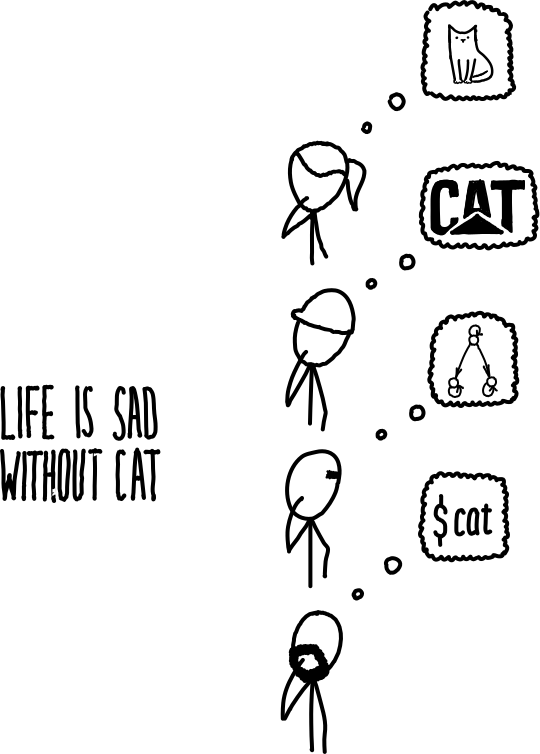
\includegraphics{/images/26-life-is-sad-without-cat.svg}
\end{figure}

The context turns the many-to-many relation between concepts and words into two maps.
The first map, \math{encode : Concept \rightarrow  Expression}, defines how the author picks words to communicate the concept.
The second map, \math{decode : Expression \rightarrow  Concept}, defines how readers interpret these words.

\section{channel}{Names as communication channels}

No matter where you go, you usually find that \href{https://en.wikipedia.org/wiki/Claude_Shannon}{Claude Shannon} was there and solved your problem fundamentally and elegantly.
Your only solace is that sometimes, his solution was not \href{https://en.wikipedia.org/wiki/Constructive_proof}{constructive}.

In information theory, a channel is a theoretical construction that allows sending messages through time and space.
A channel takes messages from a set \math{X} as inputs and produces messages from a set \math{Y} as outputs.
Channels are \em{noisy}: they distort the messages passing them; that's why the channel's input and output sets might differ.
We represent the noise mathematically by using \href{https://en.wikipedia.org/wiki/Conditional_probability}{conditional probabilities}: \math{p(y | x)} is the probability of receiving message \math{y} if the sender sent message \math{x}.

When you think of a channel, you probably imagine a cable transmitting electrical signals or how the space around you buzzes with electromagnetic waves.
Channels, however, take many forms.
Any storage device, such as a hard drive, a notebook, or the brain's memory system, is a channel transmitting messages through time.

We can view words as communication channels passing concepts from one mind to another through time.
As we saw in the \href{#maps-of-meaning}{Maps of meaning} section, these channels are fundamentally noisy: the output concept might differ from the sender's input depending on the word choice and the receiver's context.

\begin{figure}[grayscale-diagram]
  \marginnote{mn-channel}{
    Words are noisy channels transmitting concepts across minds.
    For example, when readers see the word ``index'', they can think of a pointer into an array instead of the \href{https://en.wikipedia.org/wiki/Inverted_index}{inverted index} concept the author sent.
  }
  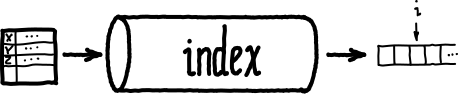
\includegraphics{/images/26-index-channel.svg}
\end{figure}

One fundamental characteristic of a channel is how much its output resembles the input.
\href{https://en.wikipedia.org/wiki/Mutual_information}{Mutual information} is the value quantifying this resemblance mathematically.

This view gives us the criteria for a good name: it's the channel maximizing mutual information.
In the following formula, \math{C\sub{s}} is the sender's concept, \math{C\sub{r}} is the receiver's concept, \math{E} is the set of all possible concept expressions, and \math{I(C\sub{r}; C\sub{s})} is the mutual information computed for expression \math{e}.

\math{best\_name(C\sub{s}) = argmax\sub{ e \in  E} I(C\sub{r}; C\sub{s}) }

The channel interpretation of names is quantitative but not particularly satisfying because it involves probabilities that are hard to compute.
Furthermore, the only way to know you've found a good expression for your concept is to compare it with all other expressions.
Could we find a more elegant way to capture the essence of a good name?

\section{names-as-galois-connections}{Names as Galois connections}
\epigraph{
  Galois connections do something really cool: they tell you the best possible way to recover data that can't be recovered.
  More precisely, they tell you the best approximation to reversing a computation that can't be reversed.
}{John Baez, \href{https://math.ucr.edu/home/baez/act_course/lecture_5.html}{Applied Category Theory Course}}

We already know that \math{encode} and \math{decode} are not perfect inverses of each other.
The next best thing we can hope for is that these maps form a relaxed version of inversion: a Galois connection.

\href{https://en.wikipedia.org/wiki/Galois_connection}{Galois connection} is a mathematical concept capturing a relationship between four objects: two partially ordered sets \math{A} and \math{B} and two monotonic maps \math{F} and \math{G} between these sets.
\href{https://en.wikipedia.org/wiki/Partially_ordered_set#Partial_orders}{Partial order} means that we can compare some elements of each set using the \math{\leq} operation that satisfies a few natural laws (\href{https://en.wikipedia.org/wiki/Reflexive_relation}{reflexivity}, \href{https://en.wikipedia.org/wiki/Antisymmetric_relation}{antisymmetry}, and \href{https://en.wikipedia.org/wiki/Transitive_relation}{transitivity}).
Not all elements must be comparable.
A function \math{F} is monotonic if it preserves relative order: if \math{x \leq  y}, then \math{F(x) \leq  F(y)}.

Functions \math{F: A \rightarrow  B} and \math{G: B \rightarrow  A} form a Galois connection if they satisfy the following relation:
\math{F(a) \leq  b \iff  a \leq  G(b)} for all \math{a \in  A} and \math{b \in  B}.

\begin{figure}[grayscale-diagram,medium-size]
  \marginnote{mn-galois-connection}{
    A Galois connection between functions \math{F} and \math{G}.
  }
  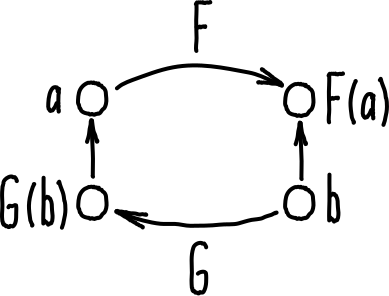
\includegraphics{/images/26-galois-connection.svg}
\end{figure}

This definition is abstract and took me a while to appreciate, so let's apply it to the problem of good names step by step.
We start with the sets in question and their orderings.

Our first set is the set of expressions \math{E}.
For expressions \math{e\sub{1}, e\sub{2} \in  E}, we say that \math{e\sub{1} \leq  e\sub{2}} if \math{e\sub{1}} at least as expressive as \math{e\sub{2}} \em{given the reader context}.
If the expressions are equally expressive, we define the shorter element as smaller.
The reader context is a crucial component of the \math{\leq} operator.
For example, ``cat'' is more expressive than ``felis catus'' in a regular conversation, but it might be the other way around in a scientific paper.
This paragraph doesn't do a good job at defining expression ordering, but it's \sc{ok}: the whole point of the Galois connection is to make expression comparison precise through its connection with better-defined objects.

Our second set is the set of concepts \math{C}.
If we have concepts \math{c\sub{1}, c\sub{2} \in  C}, we say that \math{c\sub{1} \leq  c\sub{2}} if \math{c\sub{1}} is at least as specific as \math{c\sub{2}}.
For example, \math{cat \leq  animal}: since every cat is an animal, there are at least as many animals as cats.
The idea of being more or less ``specific'' part might sound handwavy to you, but we can make it precise using methods of \href{https://en.wikipedia.org/wiki/Formal_concept_analysis}{formal concept analysis}.

The functions forming the Galois connection are the concept decoding function \math{decode : E \rightarrow  C} and the concept encoding function \math{encode : C \rightarrow  E}.
These functions are monotone because \math{encode} maps more specific concepts to more expressive names, and \math{decode} maps more expressive names to more specific concepts.
The connection becomes \math{decode(e) \leq  c \iff  e \leq  encode(c)}.

Even the specialized equivalence looks unintuitive, so let's see how it holds with an example.
Imagine we want to name a variable holding the amount of \sc{usd} in a bank account (that's our concept \math{c}).
Would \math{value} be an appropriate variable name?

Let's see what our connection tells us: \math{decode(value)} is a vague concept, less specific than the bank account balance.
Hence, \math{decode(value) > c}, so \math{value} is not a good name.
I would prefer \math{usd\_balance}, which decodes to a more specific concept.

But wait, wouldn't \math{bank_account_usd_balance} be an even better name?
It depends on the context!
A shorter name is preferable if the reader knows that we are dealing with bank accounts in a piece of code.
At least, that's how I defined the expression ordering; your mileage may vary.

\section{conclusion}{Conclusion}

In this article, we explored the difference between concepts and their expressions,
determined the crucial role of the reader's context in the interpretation,
and finished with heavy mathematical machinery that pinpoints good names using a variant of \href{https://en.wikipedia.org/wiki/Occam's_razor}{Occam's razor}:
A good name is as succinct as possible but still specific enough to convey the intended concept.

How do we apply this knowledge?
For me, the main lesson is that managing the reader's context is crucial for effective communication:

\begin{itemize}
\item
  Many resources recommend that the variable name length should be proportional to the size of the scope containing it\sidenote{mn-variable-length-scope}{
  See, for example, \href{https://google.github.io/styleguide/go/decisions.html#variable-names}{Google's Go styleguide}.
  Bob Martin mentions this rule of thumb in his book ``Clean Code''.}.
  This recommendation makes a lot of sense if we view it though the prism of context management: if the variable definition is in the view of sight, the reader won't have any trouble decoding it, no matter how short it is.
  The same idea applies to names that are part of the programming lore, such as \code{i} and \code{j} for loop counters.
\item
  Create a project glossary and make it obligatory for all contributors to read.
  Consistently use names from the glossary.
\item
  Pause and review your variable identifiers once you finished writing your code.
  What would be the decoding of each identifier if you saw it for the first time?
  Would a newhire understand these names?
\end{itemize}

Happy naming!

\section{related-work}{Related work}

``\href{https://teamscale.com/hubfs/26978363/Publications/2005-concise-and-consistent-naming.pdf}{Concise and Consistent Naming}'' by Florian Deißenböck and Markus Pizka provides a similar, though slightly simpler, formal model of variable names in section 3.2.


\end{document}